\documentclass[Lecture.tex]{subfiles}
\begin{document}
\section{2.4: The Second Derivative}
\begin{frame}{Definition}
  \begin{defn}
    If both $f$ and $f^\prime$ are differentiable functions, the {\it second derivative}, $f^{\prime\prime}$, is the derivative of $f^\prime$:
    $$f^{\prime\prime}(x) = \frac{\operatorname{d}^2}{\operatorname{dx}^2}f(x) = \ddx{x}\left(\ddx{x} f(x)\right)$$
  \end{defn}
  \onslide<2->{
    \begin{rmk}
      The second derivative tells us the rate of change of the first derivative, or the {\it acceleration}.
    \end{rmk}
  }
\end{frame}

\subsection{Concavity}

\begin{frame}{Example}
  Consider the position function 
  $$s(t) = -4.9t^2 + 9.8t.$$
  \begin{itemize}
  \item<2->
    The first derivative gives the velocity of the object at time $t$,
    $$v(t) = s^\prime(t) = -9.8t.$$
  \item<3->
    The second derivative gives the rate of change of acceleration (due to gravity)
    $$a = v^\prime(t) = s^{\prime\prime}(t) = -9.8 \frac{\text{m}}{\text{s}^2}.$$
  \end{itemize}
\end{frame}

\begin{frame}{Example (Cont.)}
  \begin{itemize}
  \item<1->
    The acceleration tells us that each second the object loses 9.8 m/s in velocity.
  \item<2->
    This fits our previous observation that the velocity is 0 when $t = 1$, at the vertex of the parabola.
  \item<3->
    By the time the object returns to its original position at $t = 2$, its speed is the same (9.8 m/s), but in the {\bf opposite} direction.
  \item<4->
    This is all observable from the graph of $s(t)$, which is a downward facing parabola.
    This is an example of a {\it concave down} function.
  \item<5->
    Clearly, an upward facing parabola should be a {\it concave up} function.
  \end{itemize}
\end{frame}

\begin{frame}{Formal Definition}
  \begin{defn}
    \begin{itemize}
    \item<1->
      If $f^{\prime\prime}(x) < 0$ on an interval, then $f^\prime(x)$ is decreasing on that interval and $f(x)$ is {\it concave down} on that interval.
    \item<2->
      If $f^{\prime\prime} > 0$ on an interval, then $f^\prime(x)$ is increasing on that interval and $f(x)$ is {\it concave up} on that interval.
    \end{itemize}
  \end{defn}
\end{frame}

\begin{frame}{Example}
  Consider the function $f(x) = (x - 2)^2 + 4$.
  \onslide<2->{
    \begin{eqnarray*}
      \onslide<2->{f^\prime(x) &=&} \onslide<3->{2(x - 2) = 2x - 4}\\
      \onslide<4->{f^{\prime\prime}(x)} \onslide<5->{&=& 2 > 0.}
    \end{eqnarray*}
  }
  \onslide<6->{Therefore, by definition, $f(x)$ is concave up.}
  \onslide<7->{
    \begin{center}
      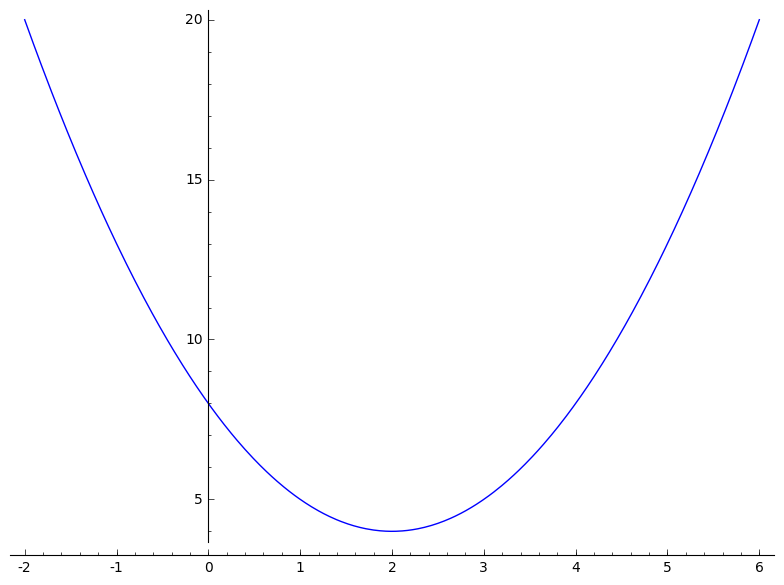
\includegraphics[scale=0.25]{concUp}
    \end{center}
    }
\end{frame}
\end{document}
